\chapter{Обзор подходов к компиляции гетерогенных приложений}\label{ch:overview}

\section{Логическая модель API для GPGPU}\label{sec:overview/api}

Память хоста.
Память устройства.
Глобальная.
Виртуальная разделяемая.
Константная.
Локальная.
Приватная.
Обычно тип памяти напрямую запрашивается при работе с API.

\begin{figure}[ht]
    \centerfloat{
        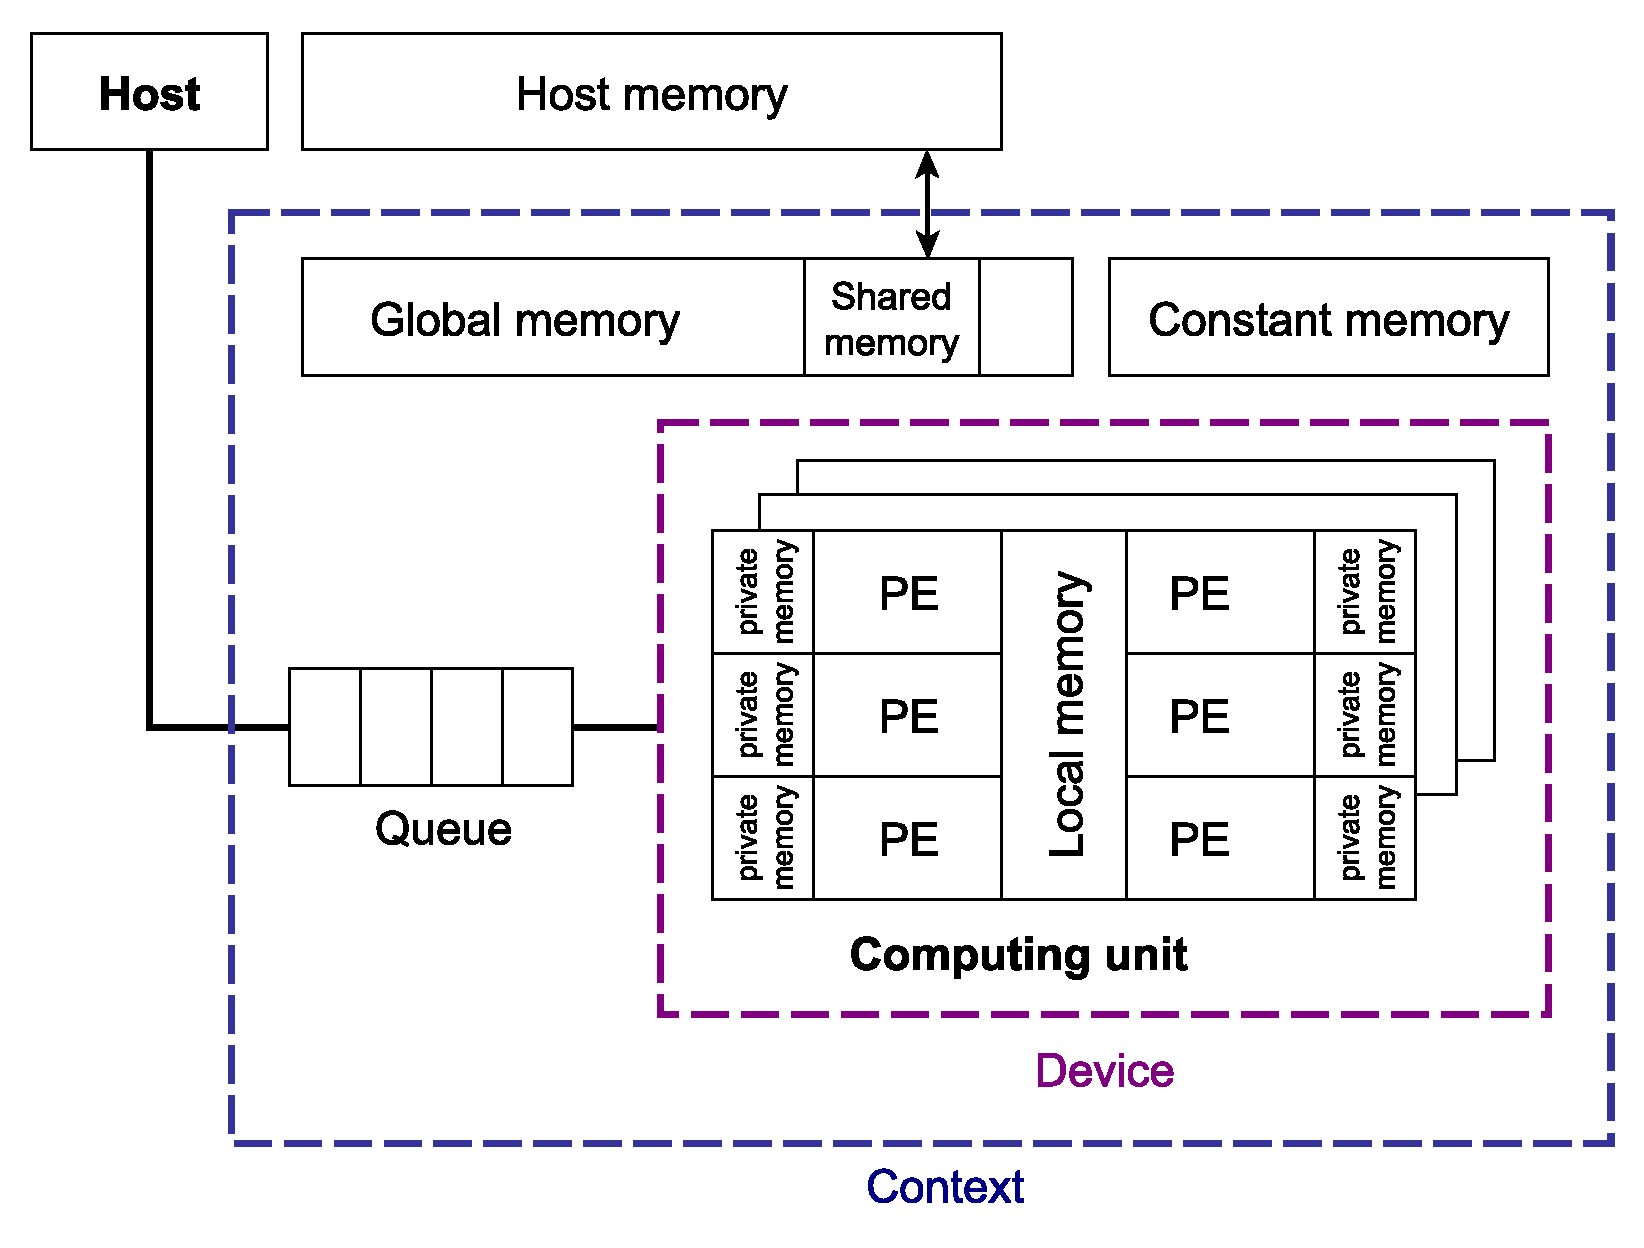
\includegraphics[scale=0.6]{Vladimirov/images/logical-memory.pdf}
    }
    \caption{Логическая модель памяти}\label{fig:logical-memory}
\end{figure}

Логическая модель памяти представлена на рисунке~\cref{fig:logical-memory}

Пробуем цитирование: \cite{Gosele1999161}

\section{Векторный характер графических систем команд}\label{sec:overview/hw}

Высокая производительность.
Отсутствие накладных расходов на переключение контекста (нет OS).
Сравнительно далёкая и дорогая память.
Часто отсутствие кешей и короткий конвейер.
Всё это мотивирует большие регистровые файлы.

\begin{figure}[ht]
    \centerfloat{
        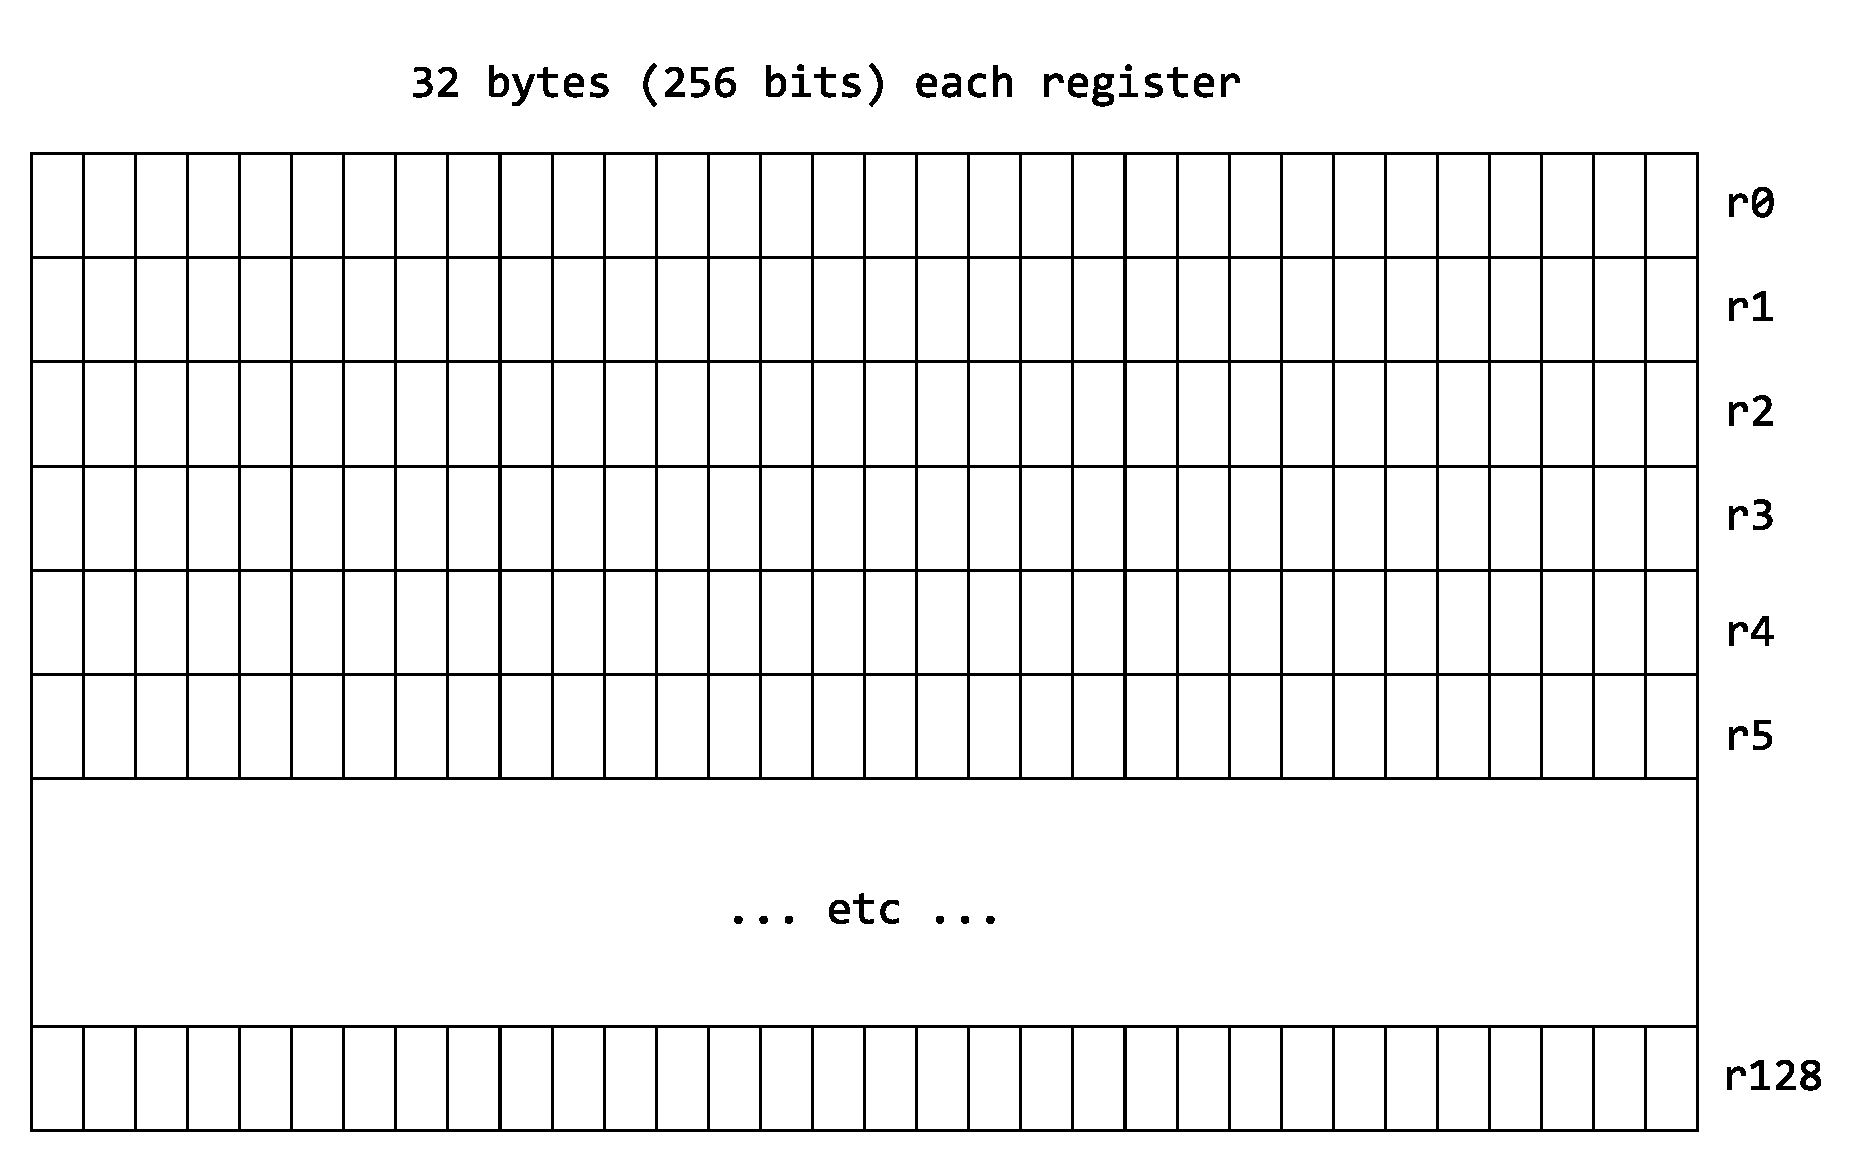
\includegraphics[scale=0.6]{Vladimirov/images/genisa-addressing-base.pdf}
    }
    \caption{Схема регистрового файла}\label{fig:genisa-addressing-base}
\end{figure}

Схема регистрового файла представлена на рисунке~\cref{fig:genisa-addressing-base}


\section{Подходы к векторизации}\label{sec:overview/vectorizing}

Скалярная ISA и скалярное API (Cuda, NVPTX). Гибкая векторизация за счёт механизмов HW.
Сложное и дорогое железо.

Векторная ISA и скалярное API (OpenCL, SYCL). Векторизация после основных оптимизаций как часть кодогенерации.
Проблемы с векторизацией внешних циклов.
Необходимость SIMDX-dispatch, влияние на распределение регистров.

Векторная ISA и векторное API (CM) с ручным управлением регистровым файлом.
Минимальная роль компилятора.
Крайне сложное программирование.


\FloatBarrier
